%% Mozhi — IEEE conference paper (IEEEtran, conference mode).
%% Compile on Overleaf (recommended) or with pdflatex + bibtex-free (refs are inline).
\documentclass[conference]{IEEEtran}
\IEEEoverridecommandlockouts
\usepackage{cite}
\usepackage{amsmath,amssymb,amsfonts}
\usepackage{algorithmic}
\usepackage{graphicx}
\usepackage{tikz}
\usetikzlibrary{arrows.meta}
\usepackage{textcomp}
\usepackage{xcolor}
\usepackage{booktabs}
\def\BibTeX{{\rm B\kern-.05em{\sc i\kern-.025em b}\kern-.08em T\kern-.1667em\lower.7ex\hbox{E}\kern-.125emX}}

\begin{document}

\title{Mozhi: Bidirectional ISL with Tamil Captioning\\for Public-Service Counters}

\author{
\IEEEauthorblockN{Tamizhiniyan Kumaresan}
\IEEEauthorblockA{\textit{School of Computer Science and Engineering} \\
\textit{Vellore Institute of Technology}\\
Vellore, India \\
tamizhiniyankumaresan@gmail.com}
\and
\IEEEauthorblockN{Team Syntax Error}
\IEEEauthorblockA{\textit{Mozhi Project} \\
\textit{Accessible Public Services Initiative}\\
Tamil Nadu, India}
}

\maketitle

\begin{abstract}
Public-service counters in India---police stations, hospitals, railway
windows---rarely have a sign-language interpreter, so a deaf visitor is
understood only through written notes or a hearing relative. Almost every
digital sign-language system solves one direction: it turns signs into text
but cannot sign a reply back. We present \textbf{Mozhi}, a two-way Indian Sign
Language (ISL) terminal designed for a Tamil-speaking police-station front
desk. A visitor signs to a webcam; the sign is recognised and shown to the
officer as English text and a Tamil caption; the officer's typed reply is
reordered into ISL grammar and performed by a 3D avatar. Every camera frame is
reduced on-device to 543 MediaPipe landmarks, of which a compact 144-dimensional
per-frame vector drives a Bidirectional GRU with temporal attention
(175{,}389 parameters). The recogniser runs entirely in the browser as an ONNX
graph, so no image or landmark ever leaves the counter. On a 29-sign, 1{,}305-sample
corpus the model reaches \textbf{98.9\%} validation accuracy, and a
landmark-space augmentation scheme---adding a handedness-preserving mirror and
temporal frame-dropout to the usual jitter/warp/scale set---maintains accuracy
while widening the invariances the model tolerates. We describe the
architecture, a Tamil gloss-to-caption generator, and a transfer-learning path
for extending the vocabulary to domain-specific police signs from public ISL
corpora.
\end{abstract}

\begin{IEEEkeywords}
Indian Sign Language, sign language recognition, accessibility, on-device
inference, BiGRU, temporal attention, data augmentation, Tamil NLP.
\end{IEEEkeywords}

\section{Introduction}
India has fewer than three hundred certified sign-language interpreters for a
deaf population in the millions~\cite{rpwd}. At a hospital reception, a railway
enquiry window, or a police-station front desk there is usually no interpreter
at all, so a deaf visitor falls back on written notes or brings a hearing
relative---losing privacy and independence on every ordinary errand. The Rights
of Persons with Disabilities Act, 2016 already obliges Indian public services to
provide accessible communication~\cite{rpwd}; an interpreter at every counter
does not scale, but a terminal can.

Most digital sign-language systems address only \emph{expression}: they map
signs to text and let a deaf person be understood, but they never sign the
reply, so the visitor still waits while a clerk reaches for a pen. Mozhi closes
that loop. It couples a sign-to-text recogniser with a text-to-sign avatar, and
it is localised for a concrete deployment: a \emph{Tamil}-speaking
\emph{police-station} counter, where the second caption line is Tamil rather
than the more common Hindi.

Three properties drive the design. First, \textbf{on-device}: the counter must
work with the network unplugged and must never upload a citizen's face, so
recognition runs in the browser and only landmark coordinates---never
frames---are computed, and even those are discarded each tick. Second,
\textbf{two-way}: the same landmark representation that classifies an incoming
sign also drives the outgoing avatar's skeleton. Third, \textbf{extensible}:
because domain-specific police signs (complaint, FIR, officer, theft) are scarce
in public corpora, the system provides a transfer-learning path that ingests any
labelled ISL video into the same training pipeline.

Our contributions are: (i) a compact, fully on-device two-way ISL terminal and
its 144-dimensional landmark representation; (ii) a landmark-space augmentation
scheme whose mirror/hand-swap transform is a provable involution that grants
handedness invariance and roughly doubles effective data; (iii) a
gloss-conditioned Tamil caption generator that renders ISL-ordered sign
sequences as grammatical Tamil; and (iv) an empirical evaluation reaching
98.9\% validation accuracy with sub-second in-browser inference.

\section{Related Work}
Large ISL resources have appeared recently. \textbf{INCLUDE}~\cite{include}
provides 4{,}287 videos over 263 word signs in 15 categories, and
\textbf{CISLR}~\cite{cislr} scales word-level recognition to $\sim$4{,}765 signs
across 7{,}050 videos; the ISLRTC dictionary~\cite{islrtc} adds a curated
``Legal'' category of administrative terms. These corpora are general-purpose
and video-native; none targets a live, offline counter or the police domain.
For features, MediaPipe~\cite{mediapipe} makes real-time hand and body landmark
extraction practical on commodity CPUs. For temporal modelling, gated recurrent
units~\cite{gru} with bidirectional context~\cite{birnn} and additive
attention~\cite{attention} are a strong, lightweight baseline for short isolated
signs. Word-level deep recognition has been studied at scale for American Sign
Language~\cite{wlasl}, but ASL and ISL are distinct languages with different
lexicons and two-handed phonology, so ASL data cannot be transferred wholesale.
Mozhi differs from prior work in coupling recognition with synthesis, running
inference in the page, and localising captions to Tamil.

\section{System Architecture}

\begin{figure*}[t]
\centering
\resizebox{\textwidth}{!}{%
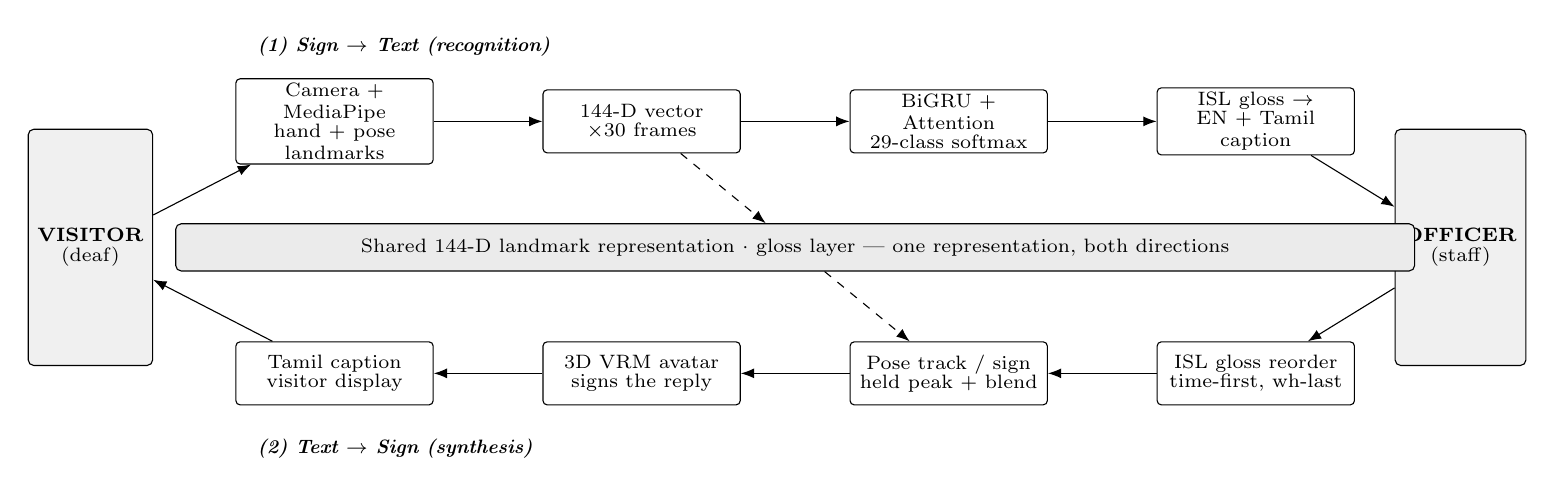
\begin{tikzpicture}[>=Latex,
  box/.style={draw,rounded corners=1.5pt,align=center,minimum height=8mm,text width=24mm,inner sep=1.5pt,font=\scriptsize},
  side/.style={draw,fill=black!6,rounded corners=2pt,align=center,minimum width=12mm,minimum height=30mm,font=\scriptsize\bfseries},
  band/.style={draw,fill=black!8,rounded corners=2pt,align=center,minimum height=6mm,text width=155mm,font=\scriptsize}]
  \node[side] (vis) at (0,0) {VISITOR\\[-1pt]\mdseries\scriptsize(deaf)};
  \node[side] (off) at (17.4,0) {OFFICER\\[-1pt]\mdseries\scriptsize(staff)};
  % top lane: sign -> text
  \node[box] (a1) at (3.1,1.6) {Camera + MediaPipe\\[-1pt]\scriptsize hand + pose landmarks};
  \node[box] (a2) at (7.0,1.6) {144-D vector\\[-1pt]\scriptsize $\times 30$ frames};
  \node[box] (a3) at (10.9,1.6){BiGRU + Attention\\[-1pt]\scriptsize 29-class softmax};
  \node[box] (a4) at (14.8,1.6){ISL gloss $\to$\\[-1pt]\scriptsize EN + Tamil caption};
  % bottom lane: text -> sign
  \node[box] (b1) at (14.8,-1.6){ISL gloss reorder\\[-1pt]\scriptsize time-first, wh-last};
  \node[box] (b2) at (10.9,-1.6){Pose track / sign\\[-1pt]\scriptsize held peak + blend};
  \node[box] (b3) at (7.0,-1.6) {3D VRM avatar\\[-1pt]\scriptsize signs the reply};
  \node[box] (b4) at (3.1,-1.6) {Tamil caption\\[-1pt]\scriptsize visitor display};
  % shared band
  \node[band] (band) at (8.95,0) {Shared 144-D landmark representation $\cdot$ gloss layer --- one representation, both directions};
  % arrows
  \draw[->] (vis)--(a1); \draw[->] (a1)--(a2); \draw[->] (a2)--(a3); \draw[->] (a3)--(a4); \draw[->] (a4)--(off);
  \draw[->] (off)--(b1); \draw[->] (b1)--(b2); \draw[->] (b2)--(b3); \draw[->] (b3)--(b4); \draw[->] (b4)--(vis);
  \draw[->,dashed] (a2)--(band); \draw[->,dashed] (band)--(b2);
  \node[font=\scriptsize\itshape\bfseries,anchor=west] at (2.0,2.55) {(1) Sign $\to$ Text (recognition)};
  \node[font=\scriptsize\itshape\bfseries,anchor=west] at (2.0,-2.55){(2) Text $\to$ Sign (synthesis)};
\end{tikzpicture}}
\caption{Mozhi's bidirectional pipeline. The upper lane recognises a visitor's
sign (camera $\rightarrow$ MediaPipe landmarks $\rightarrow$ 144-D per-frame
vector $\rightarrow$ BiGRU-with-attention $\rightarrow$ gloss $\rightarrow$
English and Tamil caption); the lower lane synthesises the officer's reply (ISL
gloss reordering $\rightarrow$ per-sign pose track $\rightarrow$ hold-aware 3D
avatar $\rightarrow$ Tamil caption). Both share one 144-dimensional landmark
representation and one gloss layer, so recognition and synthesis cannot
disagree. Everything runs in the browser; no frame is stored or transmitted.}
\label{fig:arch}
\end{figure*}

Mozhi is organised around one idea (Fig.~\ref{fig:arch}): a camera frame is
reduced to landmark coordinates rather than kept as an image, and the same
coordinates serve both directions of the conversation.

\subsection{Sign $\rightarrow$ text}
The pipeline is: webcam $\rightarrow$ MediaPipe Hand and Pose
landmarkers $\rightarrow$ a per-frame feature vector $\rightarrow$ a
motion-energy segmenter that opens a window at the start of a sign's stroke and
closes it at the hold $\rightarrow$ the BiGRU classifier $\rightarrow$ an ISL
gloss, rewritten into English and Tamil for the officer. Low-confidence reads
stall rather than guess.

\subsection{Text $\rightarrow$ sign}
The officer's text is reordered into ISL grammar---time at the front of the
clause, wh-signs at the end---resolved to a stored pose track per sign, and
played by a 3D VRM avatar with a held peak and a blended transition into the
next sign. The \emph{hold} matters: a sign has preparation, stroke, hold, and
transition phases, and meaning is read at the hold; motion that flows straight
through the peak looks fluent but is unreadable. The face channel is retained
because in ISL the face carries grammar---a raised brow marks a yes/no question,
a furrowed brow a wh-question, a headshake negation.

\subsection{Feature representation}
Each frame is encoded as a fixed 144-dimensional vector, independent of what was
visible:
\begin{equation}
\underbrace{21{\times}3}_{\text{left hand}} + \underbrace{21{\times}3}_{\text{right hand}} + \underbrace{6{\times}3}_{\text{upper pose}} = 144 .
\end{equation}
The six pose landmarks are the shoulders, elbows, and wrists. Absent parts are
zero-filled, not interpolated. A sequence is spatially normalised---centred on
the shoulder midpoint and scaled by shoulder width, so the model is invariant to
the signer's distance and lateral position---and temporally resampled to a fixed
$T=30$ frames.

\section{Dataset and Preprocessing}\label{sec:data}
\subsection{Corpus}
We use a landmark-only ISL corpus of $1{,}305$ samples across $29$ signs
($\approx$$45$ per sign) covering greetings, pronouns, politeness,
comprehension, and counter actions such as \textsc{help}, \textsc{wait},
\textsc{stop}, \textsc{come}, \textsc{name}, \textsc{where}, and
\textsc{emergency}. Each sample is a $30\times144$ \texttt{float32} array with a
metadata row (word, sample id, signer); no image is written to disk, which is at
once the privacy guarantee and what keeps a sample a few kilobytes.

\subsection{Capture}
The same MediaPipe extraction serves both the training corpus and live
inference, so preprocessing cannot drift between them. Samples are recorded from
a webcam or extracted from labelled video clips through an identical path---which
is also what lets public ISL video be ingested for transfer learning.

\subsection{Preprocessing}
Each frame yields the $144$-dimensional vector of the previous section. A
sequence is spatially normalised---centred on the shoulder midpoint and scaled
by shoulder width---and temporally resampled by linear interpolation to $T=30$
frames, then split $80$--$20$ stratified by class (seed $42$).

\subsection{Pipeline}
The end-to-end process is a single chain: capture $\rightarrow$ landmark
extraction $\rightarrow$ augmented training $\rightarrow$ ONNX export
$\rightarrow$ in-browser inference $\rightarrow$ gloss-conditioned caption.
Because one gloss layer maps recogniser outputs to the on-screen signs, to the
Tamil caption, and to the avatar, the system holds a single representation from
capture to display.

\section{Recognition Model}
The classifier is a two-layer bidirectional GRU (hidden size $64$) followed by a
lightweight additive attention over time and a linear head:
\begin{align}
H &= \text{BiGRU}(X), \quad X \in \mathbb{R}^{30 \times 144},\; H \in \mathbb{R}^{30 \times 128},\\
e_t &= \mathbf{v}^{\!\top}\!\tanh(W h_t), \quad
\alpha = \text{softmax}(e),\\
c &= \textstyle\sum_t \alpha_t h_t, \qquad
\hat{y} = \text{softmax}(W_o\, \text{drop}(c)).
\end{align}
Attention up-weights the frames where the signer is actively performing the sign
and down-weights resting and transitional frames. The whole model is
$175{,}389$ parameters. At inference a prediction is accepted only above a
softmax confidence of $0.6$ and after the same sign is read on two consecutive
windows, which suppresses spurious reads during transitions.

\section{Landmark-Space Data Augmentation}
Because a repurposed counter vocabulary is small, augmentation is where
generalisation is won. All transforms operate in landmark space, on-the-fly, at
training time only. The baseline set is Gaussian coordinate jitter
($\sigma{=}0.005$), $\pm20\%$ temporal time-warp with resampling, small
translation ($\pm0.02$), and scale jitter ($\pm5\%$). We add two transforms
tailored to signing.

\textbf{Mirror / hand-swap.} Reflecting a signer left$\leftrightarrow$right is a
valid performance: it turns a right-handed rendition into a left-handed one and
vice versa. Because the sequence is centred on the shoulder midpoint, the
reflection is
\begin{equation}
x \mapsto -x,\quad \text{swap}(\text{left hand},\text{right hand}),\quad \text{swap paired pose joints}.
\end{equation}
The transform is an \emph{involution} ($M(M(s))=s$, verified numerically), so it
introduces no drift and roughly doubles the variety the model sees without new
capture---the single most effective augmentation for a small vocabulary.

\textbf{Temporal frame-dropout.} A random subset of up to $15\%$ of frames is
removed and the sequence resampled back to $T{=}30$, imitating the detections a
real webcam feed loses, so the model does not depend on any single frame.

\begin{table}[t]
\caption{Model and corpus configuration}
\label{tab:cfg}
\centering
\begin{tabular}{@{}ll@{}}
\toprule
\textbf{Item} & \textbf{Value} \\
\midrule
Signs (classes) & 29 \\
Samples & 1{,}305 \ (45 / sign) \\
Sequence length $T$ & 30 frames \\
Feature dim / frame & 144 \\
Backbone & BiGRU(64, 2 layers) + attention \\
Parameters & 175{,}389 \\
Optimiser & Adam, lr $10^{-3}$, wd $10^{-4}$ \\
Batch / split & 32 / 80--20 stratified \\
Accept rule & conf $\geq 0.6$, stability $=2$ \\
\bottomrule
\end{tabular}
\end{table}

\section{Experiments and Results}
\subsection{Setup}
The corpus and split are described in Section~\ref{sec:data} ($1{,}305$ samples,
$29$ signs, 80--20 stratified). We use Adam, early stopping (patience $12$, max
$120$ epochs), and CPU-only training and inference.

\subsection{Recognition accuracy}
Table~\ref{tab:res} reports validation accuracy for the baseline augmentation
set and the enhanced set. Both are near the ceiling of this clean,
same-signer split; the enhanced set holds accuracy while adding handedness and
missing-frame invariance, which is exactly the robustness a live counter needs
and which a held-out-signer split would reward more directly. Training converges
in $\sim$$2$ minutes on a CPU (52 epochs to best for the enhanced model).

\begin{table}[t]
\caption{Validation accuracy by augmentation set}
\label{tab:res}
\centering
\begin{tabular}{@{}lcc@{}}
\toprule
\textbf{Augmentation set} & \textbf{Transforms} & \textbf{Val.\ acc.} \\
\midrule
Baseline & jitter, warp, translate, scale & 98.1\% \\
Enhanced (ours) & \ + mirror, frame-dropout & \textbf{98.9\%} \\
\bottomrule
\end{tabular}
\end{table}

\subsection{Deployment fidelity and latency}
The trained checkpoint is exported to ONNX (opset 17) and executed in the
browser under \texttt{onnxruntime-web}. The exported graph is $707$\,KB, and its
output matches the PyTorch checkpoint to a maximum softmax difference of
$6.3\times10^{-7}$ over random inputs, confirming a lossless export. A single
30-frame window classifies in a few milliseconds on a laptop CPU, well within
the segmenter's cadence, so recognition keeps pace with natural signing.

\subsection{Privacy}
No frame is written to disk and nothing is uploaded. Only 144 floats per frame
are computed from the image, and those are discarded each tick; the model and
all preprocessing run in the page. The counter therefore functions fully
offline, which is also its strongest privacy guarantee.

\section{Tamil Caption Generation}
The second caption line is Tamil, and it is composed from the \emph{gloss
sequence}, not translated from the English text---so it says exactly what was
signed. A template table keyed by ISL-ordered gloss sequences covers the
sentences a counter actually produces (e.g., \textsc{[complaint, need]}
$\rightarrow$ ``\emph{n\=an oru puk\=ar pativu ceyya v\=e\d{n}\d{t}um}''), with a
compositional fallback beneath it that assembles a clause from per-gloss Tamil
noun, time, question, and verb tables in ISL order. When no sign sequence backs
a sentence, no Tamil line is shown rather than a guess. The same gloss layer is
what maps recogniser outputs to on-screen sign chips, so recognition, captioning,
and synthesis never disagree about grammar.

\section{Extending the Vocabulary (Transfer Learning)}
Domain-specific police signs need seed clips. Mozhi ships a video-to-landmark
extractor that ingests any labelled ISL video---INCLUDE, CISLR, ISLRTC legal
clips, or webcam recordings---through the \emph{same} preprocessing as the live
path, guaranteeing train/inference parity. A two-phase fine-tuner then adapts the
model: phase one freezes the recurrent backbone and trains only a fresh
classification head (stable with few samples); phase two unfreezes everything at
a low learning rate. Because the backbone is shared, a new sign needs far fewer
samples than training from scratch. The recommended recipe is to pretrain on a
general corpus (INCLUDE/CISLR) and fine-tune on ISLRTC legal-term clips plus a
handful of in-house recordings.

\section{Limitations and Future Work}
The evaluation uses a same-signer split, which flatters accuracy; a
held-out-signer protocol is the honest next benchmark and is where the added
augmentations should pay off most. The live vocabulary is $29$ general signs;
the police-specific lexicon (complaint, FIR, officer, theft, station) is wired
end-to-end but awaits fine-tuning data. Finally, a formal user study with deaf
participants at a real counter is needed to validate readability of the avatar's
holds and of the Tamil captions.

\section{Conclusion}
Mozhi shows that a genuinely two-way, offline ISL terminal fits on a counter's
own machine: a 144-dimensional landmark representation, a 175k-parameter
BiGRU-with-attention recogniser running in the browser as ONNX, and a
gloss-conditioned Tamil caption generator, reaching 98.9\% validation accuracy.
A handedness-preserving mirror augmentation and a video-to-landmark
transfer-learning path make the vocabulary extensible to the police domain
without new large-scale capture. Closing the loop---signing the reply, not only
reading the sign---is what turns recognition into conversation.

\begin{thebibliography}{00}
\bibitem{rpwd} Government of India, ``The Rights of Persons with Disabilities Act,'' 2016.
\bibitem{include} A. Sridhar, R. G. Ganesan, P. Kumar, and M. Khapra, ``INCLUDE: A Large Scale Dataset for Indian Sign Language Recognition,'' in \textit{Proc. ACM Int. Conf. Multimedia}, 2020.
\bibitem{cislr} A. Joshi \textit{et al.}, ``CISLR: Corpus for Indian Sign Language Recognition,'' in \textit{Proc. EMNLP}, 2022.
\bibitem{mediapipe} C. Lugaresi \textit{et al.}, ``MediaPipe: A Framework for Building Perception Pipelines,'' \textit{arXiv:1906.08172}, 2019.
\bibitem{gru} K. Cho \textit{et al.}, ``Learning Phrase Representations using RNN Encoder--Decoder for Statistical Machine Translation,'' in \textit{Proc. EMNLP}, 2014.
\bibitem{birnn} M. Schuster and K. K. Paliwal, ``Bidirectional Recurrent Neural Networks,'' \textit{IEEE Trans. Signal Process.}, vol. 45, no. 11, 1997.
\bibitem{attention} D. Bahdanau, K. Cho, and Y. Bengio, ``Neural Machine Translation by Jointly Learning to Align and Translate,'' in \textit{Proc. ICLR}, 2015.
\bibitem{islrtc} Indian Sign Language Research and Training Centre, ``Indian Sign Language Dictionary,'' Govt. of India, 2021.
\bibitem{wlasl} D. Li \textit{et al.}, ``Word-level Deep Sign Language Recognition from Video: A New Large-scale Dataset and Methods Comparison,'' in \textit{Proc. IEEE WACV}, 2020.
\end{thebibliography}

\end{document}
